\documentclass[11pt]{article}
\usepackage{mathblatt}


\begin{document}
\pfheftstil
\pfheftkopf{Wahrscheinlichkeit}{P10}
\pfrueckblick
\begin{pfaufg}{}{1.}{}
Schreib alle zweistelligen Folgen aus den Buchstaben A und B auf (Wiederholung erlaubt).
\fusshilfe{\mbox{1:~AA, AB, BA, BB}}
\end{pfaufg}
\begin{pfaufg}{}{2.}{}
Ergänze die Tabelle Bruch | gekürzt | Prozent.
\par\smallskip\noindent \begingroup\renewcommand{\arraystretch}{1.3}\begin{tabular}{|c|c|c|}\hline \textbf{Bruch} & \textbf{gekürzt} & \textbf{Prozent} \\ \hline $\tfrac{1}{20}$ & \rule{0pt}{3ex}\hspace{1.6cm} & \rule{0pt}{3ex}\hspace{1.6cm} \\ \hline $\tfrac{1}{5}$ & \rule{0pt}{3ex}\hspace{1.6cm} & \rule{0pt}{3ex}\hspace{1.6cm} \\ \hline $\tfrac{1}{3}$ & \rule{0pt}{3ex}\hspace{1.6cm} & \rule{0pt}{3ex}\hspace{1.6cm} \\ \hline $\tfrac{3}{20}$ & \rule{0pt}{3ex}\hspace{1.6cm} & \rule{0pt}{3ex}\hspace{1.6cm} \\ \hline\end{tabular}\endgroup\par
\fusshilfe{\mbox{2:~5 \%; 20 \%; $\approx$ 33,3 \%; 15 \%}}
\end{pfaufg}
\begin{pfaufg}{}{3.}{}
Ergänze zu 1: $\tfrac{1}{8}$; $\tfrac{3}{8}$ + $\tfrac{1}{8}$; 0,7.
\fusshilfe{\mbox{3:~$\tfrac{7}{8}$; $\tfrac{1}{2}$; 0,3}}
\end{pfaufg}
\begin{pfaufg}{}{4.}{}
Berechne: $\tfrac{1}{4}$ · $\tfrac{1}{4}$; $\tfrac{2}{4}$ · $\tfrac{2}{4}$; $\tfrac{4}{16}$ + $\tfrac{1}{16}$.
\rechenplatz{1}
\fusshilfe{\mbox{4:~$\tfrac{1}{16}$; $\tfrac{1}{4}$; $\tfrac{5}{16}$}}
\end{pfaufg}
\begin{pfaufg}{}{5.}{}
In einer Schüssel liegen 16 Pfannkuchen, 2 davon mit Senf. Jemand nimmt einen mit Marmelade heraus. Wie viele liegen noch da, wie viele davon mit Senf?
\fusshilfe{\mbox{5:~15; 2}}
\end{pfaufg}
\pfstufekopf[sergebnisseaufzhlen]{Ergebnisse aufzählen}{in 1 der letzten 5 Prüfungen}
\pfgruppe{}
\begin{pfaufg}{}{6.}{}
Paul hat zwei Mützen, eine graue und eine grüne. Er hat zwei Schals, einen gelben und einen weißen. Schreibe alle Paare aus Mütze und Schal auf. Beginne mit den Paaren mit der grauen Mütze.
\rechenplatz{4}
\fusshilfe{\mbox{6:~4 Paare: , , ,}}
\end{pfaufg}
\begin{pfaufg}{}{7.}{}
Ein Eisbecher bekommt eine Sorte und eine Soße. Die Sorten sind Vanille, Schoko und Nuss. Die Soßen sind Karamell und Himbeere. Schreibe alle Becher auf. Beginne mit den Bechern mit Vanille.
\rechenplatz{4}
\fusshilfe{\mbox{7:~6 Becher: , , , , ,}}
\end{pfaufg}
\pfgruppe{}
\begin{pfaufg}{P10 ’25}{8.}{}
Bei einem Spiel werden zwei Scheiben gleichzeitig gedreht. Bleiben sie stehen, liest man an den Pfeilen erst die Ziffer der linken, dann die der rechten Scheibe ab. Im Bild entsteht so die Zahl 12. Alle Sektoren sind gleich groß. Schreib alle Zahlen auf, die beim Drehen entstehen können.
\par\smallskip\noindent 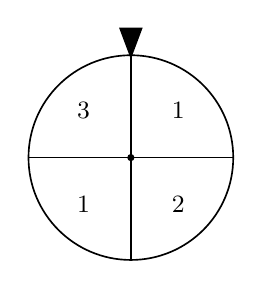
\begin{tikzpicture}[line width=0.6pt,baseline=(current bounding box.north)]\draw (0,0) circle (1.3);\draw (0,0) -- (90:1.3);\node[font=\small] at (45:0.85) {1};\draw (0,0) -- (0:1.3);\node[font=\small] at (-45:0.85) {2};\draw (0,0) -- (-90:1.3);\node[font=\small] at (-135:0.85) {1};\draw (0,0) -- (-180:1.3);\node[font=\small] at (-225:0.85) {3};\fill (0,0) circle (1.3pt);\fill (0,1.25) -- (-0.15,1.65) -- (0.15,1.65) -- cycle;\end{tikzpicture}\hspace{1.2cm}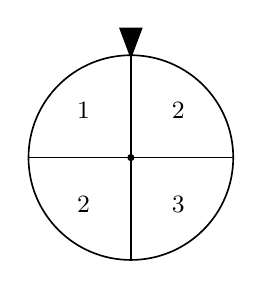
\begin{tikzpicture}[line width=0.6pt,baseline=(current bounding box.north)]\draw (0,0) circle (1.3);\draw (0,0) -- (90:1.3);\node[font=\small] at (45:0.85) {2};\draw (0,0) -- (0:1.3);\node[font=\small] at (-45:0.85) {3};\draw (0,0) -- (-90:1.3);\node[font=\small] at (-135:0.85) {2};\draw (0,0) -- (-180:1.3);\node[font=\small] at (-225:0.85) {1};\fill (0,0) circle (1.3pt);\fill (0,1.25) -- (-0.15,1.65) -- (0.15,1.65) -- cycle;\end{tikzpicture}\par
\rechenplatz{1}
\fusshilfe{\mbox{8:~11, 12, 13, 21, 22, 23, 31, 32, 33}}
\end{pfaufg}
\pfgruppe{}
\begin{pfaufg}{P10 ’17}{9.}{}
Zwei gleiche Münzen werden zusammen geworfen. Man unterscheidet, ob Zahl (Z) oder Wappen (W) oben liegt. Gib an, wie viele Ergebnisse möglich sind.
\rechenplatz{1}
\fusshilfe{\mbox{9:~4 (ZZ, ZW, WZ, WW)}}
\end{pfaufg}
\pfgruppe{}
\begin{pfaufg}{P10 ’20}{10.}{}
Wirft man einen Würfel zweimal hintereinander, gibt es 36 verschiedene Augenpaare. Dabei zählen zum Beispiel (2,1) und (1,2) als verschiedene Ergebnisse. Schreib alle Augenpaare auf, bei denen der zweite Wurf eine 2 zeigt. Ermittle die Wahrscheinlichkeit, im zweiten Wurf eine 2 zu würfeln, und gib sie in Prozent an.
\rechenplatz{2}
\fusshilfe{\mbox{10:~$\approx$ 16,7 \%}}
\end{pfaufg}
\pfsteckt{steckt auch in Nr. 44 (P10 ’18)}
\pfstufekopf[swahrscheinlichkeitan]{Wahrscheinlichkeit angeben}{in 2 der letzten 5 Prüfungen}
\pfgruppe{}
\begin{pfaufg}{}{11.}{}
Das Glücksrad im Bild hat sechs gleich große Felder. Kreuze an, welcher Anteil der Felder die 2 zeigt. 
\pfkreuzzeile{$\tfrac{1}{3}$}\pfkreuzzeile{$\tfrac{1}{2}$}
\par\smallskip\noindent \kreisdiagramm{1/1,2/1,2/1,2/1,3/1,3/1}\par
\fusshilfe{\mbox{11:~$\tfrac{1}{2}$}}
\end{pfaufg}
\begin{pfaufg}{}{12.}{}
In einer Lostrommel liegen 30 Nieten und 5 Gewinne. Gesucht ist die Wahrscheinlichkeit für einen Gewinn. Unterstreiche, was möglich und was günstig ist. Rechne nichts.
\par\noindent möglich: \leerfeld , günstig: \leerfeld \par
\fusshilfe{\mbox{12:~möglich: 35 Lose , günstig: 5 Gewinne}}
\end{pfaufg}
\pfgruppe{}
\begin{pfaufg}{P10 ’14}{13.}{}
In einer Lostrommel liegen 80 Nieten und 20 Gewinnlose. Gib die Wahrscheinlichkeit P(Gewinn) an.
\rechenplatz{1}
\fusshilfe{\mbox{13:~$\tfrac{1}{5}$ = 20 \%}}
\end{pfaufg}
\begin{pfbuendel}{gleiche Art \textperiodcentered{} 5$\times$ geprüft – kannst du überspringen}
\pfbpaar{\pfbglied{P10 ’14}{14.}{Ein Spielwürfel wird einmal geworfen. Gib die Wahrscheinlichkeit an, dass weder eine 1 noch eine 6 fällt.}{}\fusshilfe{\mbox{14:~$\tfrac{2}{3}$}}}{\pfbglied{P10 ’16}{15.}{Von 100 Energiesparlampen in einer Kiste sind 5 defekt. Eine Lampe wird herausgenommen. Gib die Wahrscheinlichkeit an, dass sie defekt ist.}{}\fusshilfe{\mbox{15:~$\tfrac{1}{20}$ = 5 \%}}}
\pfbpaar{\pfbglied{P10 ’19}{16.}{In einer Kiste liegen 20 Buntstifte: 7 grüne, 4 rote, 3 gelbe und 6 blaue. Paul greift blind einen Stift heraus und legt ihn danach zurück. Gib die Wahrscheinlichkeit an, dass er einen gelben Stift gegriffen hat.}{}\fusshilfe{\mbox{16:~$\tfrac{3}{20}$ = 15 \%}}}{\pfbglied{P10 ’24}{17.}{In Familie Siebert helfen alle 5 Kinder im Haushalt. Jede Aufgabe steht auf einem Zettel: Müll rausbringen, Spülmaschine ausräumen, Staubsaugen, Einkaufen, Joker. Wer den Joker hat, hat die Woche frei. Zu Wochenbeginn zieht jedes Kind zufällig genau einen Zettel. Gib die Wahrscheinlichkeit an, dass das erste Kind den Zettel „Staubsaugen“ zieht.}{}\fusshilfe{\mbox{17:~$\tfrac{1}{5}$ = 20 \%}}}
\end{pfbuendel}
\pfgruppe{}
\begin{pfaufg}{P10 ’15}{18.}{}
In jedem der drei Töpfe liegen sechs Kugeln. Die Wahrscheinlichkeit, blind eine weiße Kugel zu ziehen, soll 50 \% sein. Kreuze an, aus welchem Topf gezogen werden muss: Topf 1:
\pfkreuzzeile{4 weiße, 2 graue Kugeln}\pfkreuzzeile{Topf 2: 2 weiße, 4 graue Kugeln}\pfkreuzzeile{Topf 3: 3 weiße, 3 graue Kugeln}
\par\smallskip\noindent 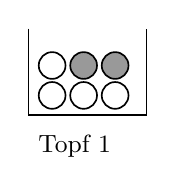
\begin{tikzpicture}[line width=0.6pt]\draw (0,1.1) -- (0,0) -- (1.5,0) -- (1.5,1.1);\draw[fill=white] (0.30,0.25) circle (0.17);\draw[fill=white] (0.70,0.25) circle (0.17);\draw[fill=white] (1.10,0.25) circle (0.17);\draw[fill=white] (0.30,0.63) circle (0.17);\draw[fill=black!40] (0.70,0.63) circle (0.17);\draw[fill=black!40] (1.10,0.63) circle (0.17);\node[font=\small] at (0.75,-0.4) {Topf 1\quad $\square$};\end{tikzpicture}\hspace{0.8cm}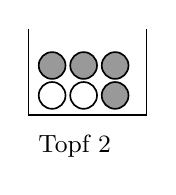
\begin{tikzpicture}[line width=0.6pt]\draw (0,1.1) -- (0,0) -- (1.5,0) -- (1.5,1.1);\draw[fill=white] (0.30,0.25) circle (0.17);\draw[fill=white] (0.70,0.25) circle (0.17);\draw[fill=black!40] (1.10,0.25) circle (0.17);\draw[fill=black!40] (0.30,0.63) circle (0.17);\draw[fill=black!40] (0.70,0.63) circle (0.17);\draw[fill=black!40] (1.10,0.63) circle (0.17);\node[font=\small] at (0.75,-0.4) {Topf 2\quad $\square$};\end{tikzpicture}\hspace{0.8cm}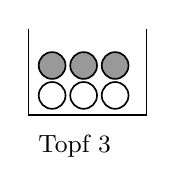
\begin{tikzpicture}[line width=0.6pt]\draw (0,1.1) -- (0,0) -- (1.5,0) -- (1.5,1.1);\draw[fill=white] (0.30,0.25) circle (0.17);\draw[fill=white] (0.70,0.25) circle (0.17);\draw[fill=white] (1.10,0.25) circle (0.17);\draw[fill=black!40] (0.30,0.63) circle (0.17);\draw[fill=black!40] (0.70,0.63) circle (0.17);\draw[fill=black!40] (1.10,0.63) circle (0.17);\node[font=\small] at (0.75,-0.4) {Topf 3\quad $\square$};\end{tikzpicture}\par
\fusshilfe{\mbox{18:~rechter Topf (3 weiße, 3 graue Kugeln)}}
\end{pfaufg}
\pfgruppe{}
\begin{pfaufg}{P10 ’17}{19.}{}
An einem Zahlenschloss lässt sich jeder der drei Ringe auf eine Ziffer von 0 bis 9 stellen. Jan stellt die ersten beiden Ringe richtig ein. Die Ziffer für den dritten Ring weiß er nicht mehr. Gib als Bruch und in Prozent an, mit welcher Wahrscheinlichkeit er sie beim ersten Versuch trifft.
\rechenplatz{1}
\fusshilfe{\mbox{19:~$\tfrac{1}{10}$ = 10 \%}}
\end{pfaufg}
\pfgruppe{}
\begin{pfaufg}{P10 ’16}{20.}{}
Mia und Lukas verkaufen Lose mit den Nummern 101 bis 900, jede Nummer genau einmal. Gezogen wird die Nummer 326. Den Hauptgewinn bekommt das Los 326. Einen Trostpreis bekommt jedes Los, das auf 26 endet, aber nicht die 326 ist. Mit einem einzigen Los gewinnt man den Hauptgewinn mit der Wahrscheinlichkeit $\tfrac{1}{800}$. Begründe das.
\par\smallskip\noindent \fbox{\parbox{6cm}{\small\textbf{Gewinnplan}\\ Hauptgewinn: Los-Nr.\ 326\\ Trostpreis: alle Lose mit der Endung 26 (außer 326)}}\par
\rechenplatz{1}
\fusshilfe{\mbox{20:~900 $-$ 101 + 1 = 800 Lose, 1 Hauptgewinn $\Rightarrow$ $\tfrac{1}{800}$}}
\end{pfaufg}
\pfgruppe{}
\begin{pfaufg}{P10 ’14}{21.}{}
Für ein Kinderfest hat Pauls Vater ein Glücksrad gebaut. In einer Spielrunde wird es zweimal nacheinander gedreht. Alle Felder sind gleich groß und werden gleich wahrscheinlich getroffen. Ermittle die Wahrscheinlichkeit, dass der Zeiger auf ein B zeigt. Gib das Ergebnis als Bruch und in Prozent an.
\par\smallskip\noindent 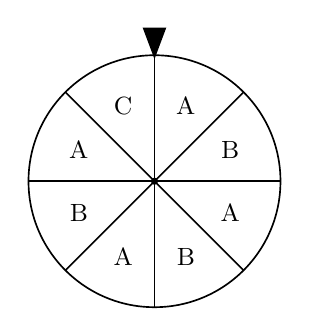
\begin{tikzpicture}[line width=0.6pt,baseline=(current bounding box.north)]\draw (0,0) circle (1.6);\draw (0,0) -- (90:1.6);\node[font=\small] at (67.5:1.04) {A};\draw (0,0) -- (45:1.6);\node[font=\small] at (22.5:1.04) {B};\draw (0,0) -- (0:1.6);\node[font=\small] at (-22.5:1.04) {A};\draw (0,0) -- (-45:1.6);\node[font=\small] at (-67.5:1.04) {B};\draw (0,0) -- (-90:1.6);\node[font=\small] at (-112.5:1.04) {A};\draw (0,0) -- (-135:1.6);\node[font=\small] at (-157.5:1.04) {B};\draw (0,0) -- (-180:1.6);\node[font=\small] at (-202.5:1.04) {A};\draw (0,0) -- (-225:1.6);\node[font=\small] at (-247.5:1.04) {C};\fill (0,0) circle (1.3pt);\fill (0,1.55) -- (-0.15,1.95) -- (0.15,1.95) -- cycle;\end{tikzpicture}\par
\rechenplatz{2}
\fusshilfe{\mbox{21:~$\tfrac{3}{8}$; 37,5 \%}}
\end{pfaufg}
\pfgruppe{}
\begin{pfaufg}{P10 ’18}{22.}{}
Eva hat 16 Pfannkuchen gebacken: 14 mit Marmelade, 2 mit Senf; von außen sieht man die Füllung nicht. Tom nimmt sich zuerst zwei, beide mit Marmelade. Pia sagt: „Jetzt greift man mit der Wahrscheinlichkeit $\tfrac{2}{16}$ einen Senf-Pfannkuchen.“ Entscheide, ob Pia recht hat, und begründe.
\rechenplatz{1}
\fusshilfe{\mbox{22:~nein, P = $\tfrac{2}{14}$ = $\tfrac{1}{7}$ $\approx$ 14,3 \%, nicht $\tfrac{2}{16}$}}
\end{pfaufg}
\pfgruppe{}
\begin{pfaufg}{VERA ’14}{23.}{}
Dose 1: 5 Vollmilch, 3 dunkle, 2 weiße Bonbons. Dose 2: 7 Vollmilch, 3 dunkle, 4 weiße. In welcher Dose ist ein dunkles beim ersten Griff wahrscheinlicher? Begründe.
\rechenplatz{2}
\fusshilfe{\mbox{23:~Dose 1: $\tfrac{3}{10}$ = 0,3 > Dose 2: $\tfrac{3}{14}$ $\approx$ 0,21}}
\end{pfaufg}
\begin{pfaufg}{P10 ’16}{\llap{\textasteriskcentered\,}24.}{}
Mia und Lukas verkaufen Lose mit den Nummern 101 bis 900, jede Nummer genau einmal. Gezogen wird die Nummer 326. Den Hauptgewinn bekommt das Los 326. Einen Trostpreis bekommt jedes Los, das auf 26 endet, aber nicht die 326 ist. Anne hat ein Los gekauft. Beim Öffnen sieht sie zuerst nur die letzte Ziffer: eine 6. Sie sagt: „Meine Chance auf einen Trostpreis liegt jetzt bei $\tfrac{7}{80}$.“ Hat Anne recht? Begründe.
\par\smallskip\noindent \fbox{\parbox{6cm}{\small\textbf{Gewinnplan}\\ Hauptgewinn: Los-Nr.\ 326\\ Trostpreis: alle Lose mit der Endung 26 (außer 326)}}\par
\rechenplatz{3}
\fusshilfe{\mbox{24:~$\tfrac{7}{80}$}}
\end{pfaufg}
\pfsteckt{steckt auch in Nr. 10 (P10 ’20)}
\pfstufekopf[sbaumergnzen]{Baum ergänzen}{in 2 der letzten 5 Prüfungen}
\pfgruppe{}
\begin{pfaufg}{}{25.}{}
In einer Dose sind 9 Kekse, 4 davon mit Schoko. Ein Schokokeks wird gegessen. Wie viele Kekse sind noch da? Wie viele davon sind mit Schoko?
\par\noindent \leerfeld[insgesamt] , davon \leerfeld \par
\fusshilfe{\mbox{25:~8 Kekse, davon 3 mit Schoko}}
\end{pfaufg}
\begin{pfaufg}{}{26.}{}
Ein Glücksrad wird zweimal gedreht. Kreuze an, ob das wie Ziehen mit oder ohne Zurücklegen ist. 
\pfkreuzzeile{mit Zurücklegen}\pfkreuzzeile{ohne Zurücklegen}
\fusshilfe{\mbox{26:~mit Zurücklegen}}
\end{pfaufg}
\pfgruppe{}
\begin{pfaufg}{P10 ’24}{27.}{}
In Familie Siebert helfen alle 5 Kinder im Haushalt. Jede Aufgabe steht auf einem Zettel: Müll rausbringen, Spülmaschine ausräumen, Staubsaugen, Einkaufen, Joker. Wer den Joker hat, hat die Woche frei. Zu Wochenbeginn zieht jedes Kind zufällig genau einen Zettel. Benjamin ist der Jüngste und zieht jede Woche als Erster aus allen fünf Zetteln. Ergänze die Wahrscheinlichkeiten im Baumdiagramm. Benjamin zieht in beiden Wochen den Joker: Weise nach, dass das die Wahrscheinlichkeit $\tfrac{1}{25}$ hat.
\par\smallskip\noindent \begin{tikzpicture}[line width=0.5pt,baseline=(current bounding box.north)]\node[font=\scriptsize,mbgrau] at (2.04,0.70) {1. Woche};\node[font=\scriptsize,mbgrau] at (5.44,0.70) {2. Woche};\fill (0,-1.35) circle (1.3pt) coordinate (k0w);\node[font=\scriptsize,inner sep=2pt] (k1) at (3.40,-0.45) {kein Joker};\node[font=\scriptsize,inner sep=2pt] (k0) at (3.40,-2.25) {Joker};\node[font=\scriptsize,inner sep=2pt] (k3) at (6.80,-1.80) {kein Joker};\node[font=\scriptsize,inner sep=2pt] (k2) at (6.80,-2.70) {Joker};\node[font=\scriptsize,inner sep=2pt] (k4) at (6.80,-0.90) {Joker};\node[font=\scriptsize,inner sep=2pt] (k5) at (6.80,0.00) {kein Joker};\draw[] (k0w) -- node[pos=0.55,anchor=south,draw,line width=0.3pt,fill=white,minimum width=0.7cm,minimum height=0.34cm,inner sep=0pt] {} (k1.west);\draw[] (k0w) -- node[pos=0.55,anchor=north,draw,line width=0.3pt,fill=white,minimum width=0.7cm,minimum height=0.34cm,inner sep=0pt] {} (k0.west);\draw[] (k0.east) -- node[pos=0.55,anchor=south,draw,line width=0.3pt,fill=white,minimum width=0.7cm,minimum height=0.34cm,inner sep=0pt] {} (k3.west);\draw[] (k0.east) -- node[pos=0.55,anchor=north,draw,line width=0.3pt,fill=white,minimum width=0.7cm,minimum height=0.34cm,inner sep=0pt] {} (k2.west);\draw[] (k1.east) -- node[pos=0.55,anchor=north,draw,line width=0.3pt,fill=white,minimum width=0.7cm,minimum height=0.34cm,inner sep=0pt] {} (k4.west);\draw[] (k1.east) -- node[pos=0.55,anchor=south,font=\scriptsize,fill=white,inner sep=1pt] {$\tfrac{4}{5}$} (k5.west);\end{tikzpicture}\par
\rechenplatz{2}
\fusshilfe{\mbox{27:~1. Woche: kein Joker 4/5, Joker $\tfrac{1}{5}$; $\tfrac{1}{25}$}}
\end{pfaufg}
\pfgruppe{}
\begin{pfaufg}{P10 ’14}{28.}{}
Für ein Kinderfest hat Pauls Vater ein Glücksrad gebaut. In einer Spielrunde wird es zweimal nacheinander gedreht. Alle Felder sind gleich groß und werden gleich wahrscheinlich getroffen. Trag im Baumdiagramm alle fehlenden Wahrscheinlichkeiten ein.
\par\smallskip\noindent \begin{tikzpicture}[line width=0.5pt,baseline=(current bounding box.north)]\node[font=\scriptsize,mbgrau] at (2.04,0.70) {1. Drehung};\node[font=\scriptsize,mbgrau] at (5.44,0.70) {2. Drehung};\fill (0,-3.80) circle (1.3pt) coordinate (k0w);\node[font=\scriptsize,inner sep=2pt] (k2) at (3.40,-6.65) {C};\node[font=\scriptsize,inner sep=2pt] (k0) at (3.40,-0.95) {A};\node[font=\scriptsize,inner sep=2pt] (k1) at (3.40,-3.80) {B};\node[font=\scriptsize,inner sep=2pt] (k6) at (6.80,-2.85) {A};\node[font=\scriptsize,inner sep=2pt] (k7) at (6.80,-3.80) {B};\node[font=\scriptsize,inner sep=2pt] (k4) at (6.80,-0.95) {B};\node[font=\scriptsize,inner sep=2pt] (k3) at (6.80,0.00) {A};\node[font=\scriptsize,inner sep=2pt] (k5) at (6.80,-1.90) {C};\node[font=\scriptsize,inner sep=2pt] (k8) at (6.80,-4.75) {C};\node[font=\scriptsize,inner sep=2pt] (k11) at (6.80,-7.60) {C};\node[font=\scriptsize,inner sep=2pt] (k9) at (6.80,-5.70) {A};\node[font=\scriptsize,inner sep=2pt] (k10) at (6.80,-6.65) {B};\draw[] (k0w) -- node[pos=0.55,anchor=north,font=\scriptsize,fill=white,inner sep=1pt] {$\tfrac{1}{8}$} (k2.west);\draw[] (k0w) -- node[pos=0.55,anchor=south,draw,line width=0.3pt,fill=white,minimum width=0.7cm,minimum height=0.34cm,inner sep=0pt] {} (k0.west);\draw[] (k0w) -- node[pos=0.55,anchor=south,draw,line width=0.3pt,fill=white,minimum width=0.7cm,minimum height=0.34cm,inner sep=0pt] {} (k1.west);\draw[] (k1.east) -- node[pos=0.55,anchor=south,draw,line width=0.3pt,fill=white,minimum width=0.7cm,minimum height=0.34cm,inner sep=0pt] {} (k6.west);\draw[] (k1.east) -- node[pos=0.55,anchor=north,draw,line width=0.3pt,fill=white,minimum width=0.7cm,minimum height=0.34cm,inner sep=0pt] {} (k7.west);\draw[] (k0.east) -- node[pos=0.55,anchor=north,draw,line width=0.3pt,fill=white,minimum width=0.7cm,minimum height=0.34cm,inner sep=0pt] {} (k4.west);\draw[] (k0.east) -- node[pos=0.55,anchor=south,draw,line width=0.3pt,fill=white,minimum width=0.7cm,minimum height=0.34cm,inner sep=0pt] {} (k3.west);\draw[] (k0.east) -- node[pos=0.55,anchor=north,draw,line width=0.3pt,fill=white,minimum width=0.7cm,minimum height=0.34cm,inner sep=0pt] {} (k5.west);\draw[] (k1.east) -- node[pos=0.55,anchor=north,draw,line width=0.3pt,fill=white,minimum width=0.7cm,minimum height=0.34cm,inner sep=0pt] {} (k8.west);\draw[] (k2.east) -- node[pos=0.55,anchor=north,draw,line width=0.3pt,fill=white,minimum width=0.7cm,minimum height=0.34cm,inner sep=0pt] {} (k11.west);\draw[] (k2.east) -- node[pos=0.55,anchor=south,draw,line width=0.3pt,fill=white,minimum width=0.7cm,minimum height=0.34cm,inner sep=0pt] {} (k9.west);\draw[] (k2.east) -- node[pos=0.55,anchor=south,draw,line width=0.3pt,fill=white,minimum width=0.7cm,minimum height=0.34cm,inner sep=0pt] {} (k10.west);\end{tikzpicture}\par
\rechenplatz{1}
\fusshilfe{\mbox{28:~1. Stufe A 1/2, B $\tfrac{3}{8}$; 2. Stufe je Ast A 1/2, B 3/8, C $\tfrac{1}{8}$}}
\end{pfaufg}
\begin{pfaufg}{BY ’23}{29.}{}
In einem Restaurant gehen 35 \% der Reservierungen telefonisch ein (T), der Rest über die Homepage (H). Bei 18 \% der Anrufe passiert ein Fehler (F). Bei der Homepage passiert in p \% der Fälle ein Fehler. Sonst klappt alles (oF). Zeichne ein Baumdiagramm mit allen Anteilen.
\rechenplatz{2}
\fusshilfe{\mbox{29:~nach H: F p/100, oF 1 $-$ p/100}}
\end{pfaufg}
\pfgruppe{}
\begin{pfaufg}{P10 ’19}{\llap{\textasteriskcentered\,}30.}{}
In einer Kiste liegen 20 Buntstifte: 7 grüne, 4 rote, 3 gelbe und 6 blaue. Marie nimmt aus der vollen Kiste blind nacheinander drei Stifte heraus und legt keinen zurück. Ergänze im Baumdiagramm die Wahrscheinlichkeiten an den zwei leeren Stellen. Entscheide für den fett gezeichneten Pfad, ob die Aussagen wahr oder falsch sind, und kreuze an:
\par\smallskip\noindent \begin{tikzpicture}[line width=0.5pt,baseline=(current bounding box.north)]\node[font=\scriptsize,mbgrau] at (1.80,0.70) {1. Stift};\node[font=\scriptsize,mbgrau] at (4.80,0.70) {2. Stift};\node[font=\scriptsize,mbgrau] at (7.80,0.70) {3. Stift};\fill (0,-2.17) circle (1.3pt) coordinate (k0w);\node[font=\scriptsize,inner sep=2pt] (k0) at (3.00,-3.41) {nicht rot};\node[font=\scriptsize,inner sep=2pt] (k1) at (3.00,-0.93) {rot};\node[font=\scriptsize,inner sep=2pt] (k3) at (6.00,-2.79) {rot};\node[font=\scriptsize,inner sep=2pt] (k4) at (6.00,-1.55) {nicht rot};\node[font=\scriptsize,inner sep=2pt] (k5) at (6.00,-0.31) {rot};\node[font=\scriptsize,inner sep=2pt] (k2) at (6.00,-4.03) {nicht rot};\node[font=\scriptsize,inner sep=2pt] (k6) at (9.00,-4.34) {nicht rot};\node[font=\scriptsize,inner sep=2pt] (k10) at (9.00,-1.86) {nicht rot};\node[font=\scriptsize,inner sep=2pt] (k7) at (9.00,-3.72) {rot};\node[font=\scriptsize,inner sep=2pt] (k11) at (9.00,-1.24) {rot};\node[font=\scriptsize,inner sep=2pt] (k8) at (9.00,-3.10) {nicht rot};\node[font=\scriptsize,inner sep=2pt] (k13) at (9.00,0.00) {rot};\node[font=\scriptsize,inner sep=2pt] (k9) at (9.00,-2.48) {rot};\node[font=\scriptsize,inner sep=2pt] (k12) at (9.00,-0.62) {nicht rot};\draw[] (k0w) -- node[pos=0.55,anchor=north,draw,line width=0.3pt,fill=white,minimum width=0.7cm,minimum height=0.34cm,inner sep=0pt] {} (k0.west);\draw[line width=1.4pt] (k0w) -- node[pos=0.55,anchor=south,font=\scriptsize,fill=white,inner sep=1pt] {$\tfrac{4}{20}$} (k1.west);\draw[] (k0.east) --  (k3.west);\draw[] (k1.east) --  (k4.west);\draw[line width=1.4pt] (k1.east) -- node[pos=0.55,anchor=south,font=\scriptsize,fill=white,inner sep=1pt] {$\tfrac{3}{19}$} (k5.west);\draw[] (k0.east) --  (k2.west);\draw[] (k2.east) --  (k6.west);\draw[] (k4.east) --  (k10.west);\draw[] (k2.east) --  (k7.west);\draw[] (k4.east) --  (k11.west);\draw[] (k3.east) --  (k8.west);\draw[line width=1.4pt] (k5.east) -- node[pos=0.55,anchor=south,font=\scriptsize,fill=white,inner sep=1pt] {$\tfrac{2}{18}$} (k13.west);\draw[] (k3.east) -- node[pos=0.55,anchor=south,draw,line width=0.3pt,fill=white,minimum width=0.7cm,minimum height=0.34cm,inner sep=0pt] {} (k9.west);\draw[] (k5.east) --  (k12.west);\end{tikzpicture}
\par\smallskip\noindent \begingroup\renewcommand{\arraystretch}{1.5}\begin{tabular}{|p{8.0cm}|c|c|}\hline Aussage & wahr & falsch \\ \hline „Marie zieht drei Stifte mit verschiedenen Farben.“ & $\square$ & $\square$ \\ \hline „Marie legt jeden Stift nach dem Ziehen zurück.“ & $\square$ & $\square$ \\ \hline „Der fette Pfad hat eine Wahrscheinlichkeit unter 1 \%.“ & $\square$ & $\square$ \\ \hline\end{tabular}\endgroup\par
\fusshilfe{\mbox{30:~$\tfrac{16}{20}$; $\tfrac{3}{18}$; Aussage 1 falsch, 2 falsch, 3 wahr}}
\end{pfaufg}
\pfgruppe{}
\begin{pfaufg}{P10 ’20}{\llap{\textasteriskcentered\,}31.}{}
Wirft man einen Würfel zweimal hintereinander, gibt es 36 verschiedene Augenpaare. Dabei zählen zum Beispiel (2,1) und (1,2) als verschiedene Ergebnisse. Lisa und Max wollen ins Kino. Lisa würfelt dreimal hintereinander. Fällt dabei mindestens zweimal eine 6, bezahlt Max beide Karten. Vervollständige das Baumdiagramm. Berechne die Wahrscheinlichkeit, dass Max die Karten bezahlt.
\par\smallskip\noindent \begin{tikzpicture}[line width=0.5pt,baseline=(current bounding box.north)]\node[font=\scriptsize,mbgrau] at (1.80,0.70) {1. Wurf};\node[font=\scriptsize,mbgrau] at (4.80,0.70) {2. Wurf};\node[font=\scriptsize,mbgrau] at (7.80,0.70) {3. Wurf};\fill (0,-2.17) circle (1.3pt) coordinate (k0w);\node[font=\scriptsize,inner sep=2pt] (k0) at (3.00,-0.93) {6};\node[font=\scriptsize,inner sep=2pt] (k1) at (3.00,-3.41) {keine 6};\node[font=\scriptsize,inner sep=2pt] (k3) at (6.00,-1.55) {keine 6};\node[font=\scriptsize,inner sep=2pt] (k5) at (6.00,-4.03) {keine 6};\node[font=\scriptsize,inner sep=2pt] (k2) at (6.00,-0.31) {6};\node[font=\scriptsize,inner sep=2pt] (k4) at (6.00,-2.79) {6};\node[font=\scriptsize,inner sep=2pt] (k9) at (9.00,-1.86) {keine 6};\node[font=\scriptsize,inner sep=2pt] (k13) at (9.00,-4.34) {keine 6};\node[font=\scriptsize,inner sep=2pt] (k8) at (9.00,-1.24) {6};\node[font=\scriptsize,inner sep=2pt] (k12) at (9.00,-3.72) {6};\node[font=\scriptsize,inner sep=2pt] (k7) at (9.00,-0.62) {keine 6};\node[font=\scriptsize,inner sep=2pt] (k11) at (9.00,-3.10) {keine 6};\node[font=\scriptsize,inner sep=2pt] (k6) at (9.00,0.00) {6};\node[font=\scriptsize,inner sep=2pt] (k10) at (9.00,-2.48) {6};\draw[] (k0w) -- node[pos=0.55,anchor=south,draw,line width=0.3pt,fill=white,minimum width=0.7cm,minimum height=0.34cm,inner sep=0pt] {} (k0.west);\draw[] (k0w) -- node[pos=0.55,anchor=north,draw,line width=0.3pt,fill=white,minimum width=0.7cm,minimum height=0.34cm,inner sep=0pt] {} (k1.west);\draw[] (k0.east) -- node[pos=0.55,anchor=north,draw,line width=0.3pt,fill=white,minimum width=0.7cm,minimum height=0.34cm,inner sep=0pt] {} (k3.west);\draw[] (k1.east) -- node[pos=0.55,anchor=north,draw,line width=0.3pt,fill=white,minimum width=0.7cm,minimum height=0.34cm,inner sep=0pt] {} (k5.west);\draw[] (k0.east) -- node[pos=0.55,anchor=south,draw,line width=0.3pt,fill=white,minimum width=0.7cm,minimum height=0.34cm,inner sep=0pt] {} (k2.west);\draw[] (k1.east) -- node[pos=0.55,anchor=south,draw,line width=0.3pt,fill=white,minimum width=0.7cm,minimum height=0.34cm,inner sep=0pt] {} (k4.west);\draw[] (k3.east) -- node[pos=0.55,anchor=north,draw,line width=0.3pt,fill=white,minimum width=0.7cm,minimum height=0.34cm,inner sep=0pt] {} (k9.west);\draw[] (k5.east) -- node[pos=0.55,anchor=north,draw,line width=0.3pt,fill=white,minimum width=0.7cm,minimum height=0.34cm,inner sep=0pt] {} (k13.west);\draw[] (k3.east) -- node[pos=0.55,anchor=south,draw,line width=0.3pt,fill=white,minimum width=0.7cm,minimum height=0.34cm,inner sep=0pt] {} (k8.west);\draw[] (k5.east) -- node[pos=0.55,anchor=south,draw,line width=0.3pt,fill=white,minimum width=0.7cm,minimum height=0.34cm,inner sep=0pt] {} (k12.west);\draw[] (k2.east) -- node[pos=0.55,anchor=north,draw,line width=0.3pt,fill=white,minimum width=0.7cm,minimum height=0.34cm,inner sep=0pt] {} (k7.west);\draw[] (k4.east) -- node[pos=0.55,anchor=north,draw,line width=0.3pt,fill=white,minimum width=0.7cm,minimum height=0.34cm,inner sep=0pt] {} (k11.west);\draw[] (k2.east) -- node[pos=0.55,anchor=south,draw,line width=0.3pt,fill=white,minimum width=0.7cm,minimum height=0.34cm,inner sep=0pt] {} (k6.west);\draw[] (k4.east) -- node[pos=0.55,anchor=south,draw,line width=0.3pt,fill=white,minimum width=0.7cm,minimum height=0.34cm,inner sep=0pt] {} (k10.west);\end{tikzpicture}\par
\rechenplatz{4}
\fusshilfe{\mbox{31:~Äste 6: 1/6, keine 6: $\tfrac{5}{6}$; $\tfrac{2}{27}$ $\approx$ 7,4 \%}}
\end{pfaufg}
\pfgruppe{}
\begin{pfaufg}{P10 ’15}{\llap{\textasteriskcentered\,}32.}{}
Beim Elfmetertraining stehen 11 Spieler bereit. Jeder schießt höchstens einmal; die Reihenfolge wird ausgelost. Die Fans wünschen sich, dass ihr Torjäger Ronny unter den ersten drei Schützen ist. Vervollständige das Baumdiagramm (R: Ronny schießt, nR: Ronny schießt nicht) und trag die fehlenden Wahrscheinlichkeiten ein. Berechne die Wahrscheinlichkeit, dass Ronny unter den ersten drei Schützen ist.
\par\smallskip\noindent \begin{tikzpicture}[line width=0.5pt,baseline=(current bounding box.north)]\node[font=\scriptsize,mbgrau] at (1.80,0.70) {1. Schütze};\node[font=\scriptsize,mbgrau] at (4.80,0.70) {2. Schütze};\node[font=\scriptsize,mbgrau] at (7.80,0.70) {3. Schütze};\fill (0,-0.79) circle (1.3pt) coordinate (k0w);\node[font=\scriptsize,inner sep=2pt] (k1) at (3.00,-1.57) {nR};\node[font=\scriptsize,inner sep=2pt] (k0) at (3.00,0.00) {R};\node[font=\scriptsize,inner sep=2pt] (k2) at (6.00,-0.90) {R};\node[font=\scriptsize,inner sep=2pt] (k3) at (6.00,-2.25) {nR};\node[font=\scriptsize,inner sep=2pt] (k4) at (9.00,-1.80) {R};\node[font=\scriptsize,inner sep=2pt] (k5) at (9.00,-2.70) {nR};\draw[] (k0w) -- node[pos=0.55,anchor=north,draw,line width=0.3pt,fill=white,minimum width=0.7cm,minimum height=0.34cm,inner sep=0pt] {} (k1.west);\draw[] (k0w) -- node[pos=0.55,anchor=south,font=\scriptsize,fill=white,inner sep=1pt] {$\tfrac{1}{11}$} (k0.west);\draw[] (k1.east) -- node[pos=0.55,anchor=south,draw,line width=0.3pt,fill=white,minimum width=0.7cm,minimum height=0.34cm,inner sep=0pt] {} (k2.west);\draw[] (k1.east) -- node[pos=0.55,anchor=north,font=\scriptsize,fill=white,inner sep=1pt] {$\tfrac{9}{10}$} (k3.west);\draw[] (k3.east) -- node[pos=0.55,anchor=south,draw,line width=0.3pt,fill=white,minimum width=0.7cm,minimum height=0.34cm,inner sep=0pt] {} (k4.west);\draw[] (k3.east) -- node[pos=0.55,anchor=north,draw,line width=0.3pt,fill=white,minimum width=0.7cm,minimum height=0.34cm,inner sep=0pt] {} (k5.west);\end{tikzpicture}\par
\rechenplatz{4}
\fusshilfe{\mbox{32:~10/11, 1/10, 1/9, $\tfrac{8}{9}$; $\tfrac{3}{11}$ $\approx$ 0,27}}
\end{pfaufg}
\pfstufekopf[spfadregel]{Pfadregel}{in 3 der letzten 5 Prüfungen}
\pfgruppe{}
\begin{pfaufg}{}{33.}{}
Ein Würfel wird zweimal geworfen. Das Ereignis heißt „mindestens eine Sechs“. Nenne das Gegenereignis.
\rechenplatz{1}
\fusshilfe{\mbox{33:~Gegenereignis: keine Sechs in beiden Würfen}}
\end{pfaufg}
\begin{pfaufg}{}{34.}{}
Der Baum zeigt zweimaliges Drehen eines Glücksrads. Schreibe alle Pfade auf, die zum Ereignis „genau einmal Rot“ gehören. Rechne nichts.
\par\smallskip\noindent \baumzwei{rot/,blau/}{rot/,blau/}{rot/,blau/}\par
\rechenplatz{4}
\fusshilfe{\mbox{34:~2 Pfade: ,}}
\end{pfaufg}
\pfgruppe{}
\begin{pfaufg}{P10 ’25}{35.}{}
Bei einem Spiel werden zwei Scheiben gleichzeitig gedreht. Bleiben sie stehen, liest man an den Pfeilen erst die Ziffer der linken, dann die der rechten Scheibe ab. Im Bild entsteht so die Zahl 12. Alle Sektoren sind gleich groß. Berechne die Wahrscheinlichkeit, eine 33 zu drehen. Esra sagt: „Eine 22 ist genauso wahrscheinlich wie eine 33.“ Entscheide, ob Esra recht hat, und begründe.
\par\smallskip\noindent 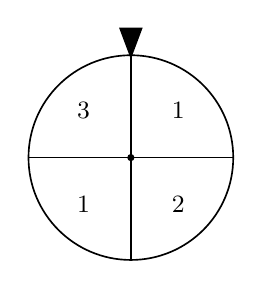
\begin{tikzpicture}[line width=0.6pt,baseline=(current bounding box.north)]\draw (0,0) circle (1.3);\draw (0,0) -- (90:1.3);\node[font=\small] at (45:0.85) {1};\draw (0,0) -- (0:1.3);\node[font=\small] at (-45:0.85) {2};\draw (0,0) -- (-90:1.3);\node[font=\small] at (-135:0.85) {1};\draw (0,0) -- (-180:1.3);\node[font=\small] at (-225:0.85) {3};\fill (0,0) circle (1.3pt);\fill (0,1.25) -- (-0.15,1.65) -- (0.15,1.65) -- cycle;\end{tikzpicture}\hspace{1.2cm}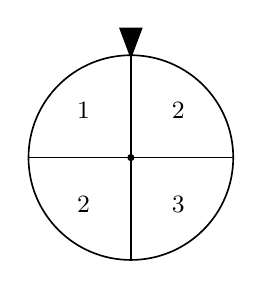
\begin{tikzpicture}[line width=0.6pt,baseline=(current bounding box.north)]\draw (0,0) circle (1.3);\draw (0,0) -- (90:1.3);\node[font=\small] at (45:0.85) {2};\draw (0,0) -- (0:1.3);\node[font=\small] at (-45:0.85) {3};\draw (0,0) -- (-90:1.3);\node[font=\small] at (-135:0.85) {2};\draw (0,0) -- (-180:1.3);\node[font=\small] at (-225:0.85) {1};\fill (0,0) circle (1.3pt);\fill (0,1.25) -- (-0.15,1.65) -- (0.15,1.65) -- cycle;\end{tikzpicture}\par
\rechenplatz{3}
\fusshilfe{\mbox{35:~$\tfrac{1}{16}$; $\tfrac{1}{8}$ $\neq$ $\tfrac{1}{16}$}}
\end{pfaufg}
\pfgruppe{}
\begin{pfaufg}{HH ’26}{36.}{}
Ein Übersetzungsprogramm übersetzt einen Satz mit 60 \% richtig. Es übersetzt zwei Sätze. Ermittle die Wahrscheinlichkeit, dass genau einer richtig ist.
\rechenplatz{2}
\fusshilfe{\mbox{36:~0,6 · 0,4 + 0,4 · 0,6 = 0,48 = 48 \%}}
\end{pfaufg}
\pfgruppe{}
\begin{pfaufg}{P10 ’20}{37.}{}
Wirft man einen Würfel zweimal hintereinander, gibt es 36 verschiedene Augenpaare. Dabei zählen zum Beispiel (2,1) und (1,2) als verschiedene Ergebnisse. Max sagt: „Zwei gleiche Augenzahlen zu werfen ist wahrscheinlicher, als im ersten Wurf eine 6 zu werfen.“ Kreuze an:
\pfkreuzzeile{Max hat recht}\pfkreuzzeile{Max hat nicht recht. Begründe deine Entscheidung}
\rechenplatz{2}
\fusshilfe{\mbox{37:~Max hat nicht Recht; beide Wahrscheinlichkeiten $\tfrac{1}{6}$}}
\end{pfaufg}
\pfgruppe{}
\begin{pfaufg}{P10 ’25}{\llap{\textasteriskcentered\,}38.}{}
Bei einem Spiel werden zwei Scheiben gleichzeitig gedreht. Bleiben sie stehen, liest man an den Pfeilen erst die Ziffer der linken, dann die der rechten Scheibe ab. Im Bild entsteht so die Zahl 12. Alle Sektoren sind gleich groß. Bestimme die Wahrscheinlichkeit, eine 12 oder eine 21 zu drehen.
\par\smallskip\noindent 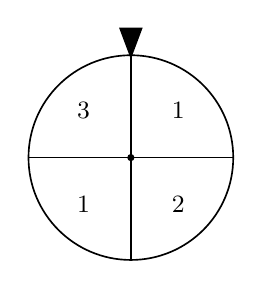
\begin{tikzpicture}[line width=0.6pt,baseline=(current bounding box.north)]\draw (0,0) circle (1.3);\draw (0,0) -- (90:1.3);\node[font=\small] at (45:0.85) {1};\draw (0,0) -- (0:1.3);\node[font=\small] at (-45:0.85) {2};\draw (0,0) -- (-90:1.3);\node[font=\small] at (-135:0.85) {1};\draw (0,0) -- (-180:1.3);\node[font=\small] at (-225:0.85) {3};\fill (0,0) circle (1.3pt);\fill (0,1.25) -- (-0.15,1.65) -- (0.15,1.65) -- cycle;\end{tikzpicture}\hspace{1.2cm}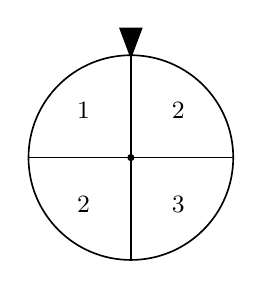
\begin{tikzpicture}[line width=0.6pt,baseline=(current bounding box.north)]\draw (0,0) circle (1.3);\draw (0,0) -- (90:1.3);\node[font=\small] at (45:0.85) {2};\draw (0,0) -- (0:1.3);\node[font=\small] at (-45:0.85) {3};\draw (0,0) -- (-90:1.3);\node[font=\small] at (-135:0.85) {2};\draw (0,0) -- (-180:1.3);\node[font=\small] at (-225:0.85) {1};\fill (0,0) circle (1.3pt);\fill (0,1.25) -- (-0.15,1.65) -- (0.15,1.65) -- cycle;\end{tikzpicture}\par
\rechenplatz{3}
\fusshilfe{\mbox{38:~$\tfrac{5}{16}$ = 31,25 \%}}
\end{pfaufg}
\pfgruppe{}
\begin{pfaufg}{P10 ’14}{\llap{\textasteriskcentered\,}39.}{}
Für ein Kinderfest hat Pauls Vater ein Glücksrad gebaut. In einer Spielrunde wird es zweimal nacheinander gedreht. Alle Felder sind gleich groß und werden gleich wahrscheinlich getroffen. Berechne die Wahrscheinlichkeit, dass der Zeiger bei beiden Drehungen auf denselben Buchstaben zeigt.
\par\smallskip\noindent 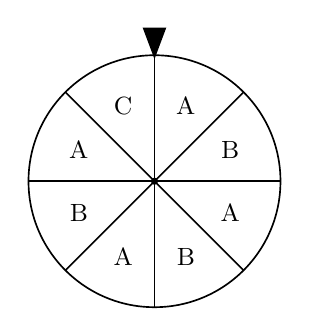
\begin{tikzpicture}[line width=0.6pt,baseline=(current bounding box.north)]\draw (0,0) circle (1.6);\draw (0,0) -- (90:1.6);\node[font=\small] at (67.5:1.04) {A};\draw (0,0) -- (45:1.6);\node[font=\small] at (22.5:1.04) {B};\draw (0,0) -- (0:1.6);\node[font=\small] at (-22.5:1.04) {A};\draw (0,0) -- (-45:1.6);\node[font=\small] at (-67.5:1.04) {B};\draw (0,0) -- (-90:1.6);\node[font=\small] at (-112.5:1.04) {A};\draw (0,0) -- (-135:1.6);\node[font=\small] at (-157.5:1.04) {B};\draw (0,0) -- (-180:1.6);\node[font=\small] at (-202.5:1.04) {A};\draw (0,0) -- (-225:1.6);\node[font=\small] at (-247.5:1.04) {C};\fill (0,0) circle (1.3pt);\fill (0,1.55) -- (-0.15,1.95) -- (0.15,1.95) -- cycle;\end{tikzpicture}\par
\rechenplatz{3}
\fusshilfe{\mbox{39:~$\tfrac{13}{32}$ $\approx$ 0,41}}
\end{pfaufg}
\pfsteckt{steckt auch in Nr. 31 (P10 ’20); Nr. 27 (P10 ’24); Nr. 48 (P10 ’25)}
\pfstufekopf[sohnezurcklegen]{ohne Zurücklegen}{in 1 der letzten 5 Prüfungen}
\pfgruppe{}
\begin{pfaufg}{}{40.}{}
Tim dreht ein Glücksrad einmal. Kreuze an, wie viele Stufen der Versuch hat. Rechne nichts. 
\pfkreuzzeile{eine Stufe}\pfkreuzzeile{zwei Stufen}\pfkreuzzeile{drei Stufen}
\fusshilfe{\mbox{40:~eine Stufe}}
\end{pfaufg}
\pfgruppe{}
\begin{pfaufg}{P10 ’24}{\llap{\textasteriskcentered\,}41.}{}
In Familie Siebert helfen alle 5 Kinder im Haushalt. Jede Aufgabe steht auf einem Zettel: Müll rausbringen, Spülmaschine ausräumen, Staubsaugen, Einkaufen, Joker. Wer den Joker hat, hat die Woche frei. Zu Wochenbeginn zieht jedes Kind zufällig genau einen Zettel. Klara zieht immer als Zweite, direkt nach Benjamin. Ermittle, mit welcher Wahrscheinlichkeit Klara in Woche 1 den Joker bekommt.
\rechenplatz{2}
\fusshilfe{\mbox{41:~$\tfrac{1}{5}$}}
\end{pfaufg}
\pfgruppe{}
\begin{pfaufg}{NI ’25}{42.}{}
Von 72 Schokoladeneiern mit 10 Sammelfiguren hat Elena 7 gekauft, darin 2 Figuren. Wie wahrscheinlich enthält das nächste Ei eine Figur?
\fusshilfe{\mbox{42:~P = $\tfrac{8}{65}$ $\approx$ 12,31 \%}}
\end{pfaufg}
\pfgruppe{}
\begin{pfaufg}{P10 ’19}{\llap{\textasteriskcentered\,}43.}{}
In einer Kiste liegen 20 Buntstifte: 7 grüne, 4 rote, 3 gelbe und 6 blaue. Marc sagt: „Zieht man ohne Zurücklegen drei Stifte aus der Kiste, ist es doppelt so wahrscheinlich, drei blaue zu bekommen wie drei gelbe.“ Zeige mit einer Rechnung, dass Marc sich irrt.
\rechenplatz{3}
\fusshilfe{\mbox{43:~20-mal so hoch, Behauptung falsch}}
\end{pfaufg}
\pfgruppe{}
\begin{pfaufg}{P10 ’18}{\llap{\textasteriskcentered\,}44.}{}
Für ein anderes Fest backt Eva wieder 14 Pfannkuchen mit Marmelade (M) und 2 mit Senf (S). Der erste Gast nimmt blind nacheinander zwei Pfannkuchen. Er erwischt mindestens einen mit Senf: Nenne alle Ergebnisse, die dafür in Frage kommen. Ermittle die Wahrscheinlichkeit, dass beide Pfannkuchen des ersten Gastes Marmelade enthalten. Beschreibe in Worten das Ereignis E, dessen Wahrscheinlichkeit diese Rechnung angibt: $P(E) = \tfrac{2}{16}\cdot\tfrac{1}{15} + \tfrac{14}{16}\cdot\tfrac{13}{15}$
\rechenplatz{3}
\fusshilfe{\mbox{44:~(S | M), (M | S), (S | S); $\approx$ 0,758}}
\end{pfaufg}
\pfsteckt{steckt auch in Nr. 32 (P10 ’15); Nr. 30 (P10 ’19)}
\pfstufekopf[sgegenereignis]{Gegenereignis}{in 1 der letzten 5 Prüfungen}
\pfgruppe{}
\begin{pfaufg}{}{45.}{}
Ein Würfel wird einmal geworfen. Wie groß ist die Wahrscheinlichkeit, dass weder 2 noch 3 noch 4 fällt?
\rechenplatz{2}
\fusshilfe{\mbox{45:~$\tfrac{1}{2}$}}
\end{pfaufg}
\par\Needspace*{0.55\textheight}\pfstufekopf[serkennen1]{Was ist gesucht?}{}
\begin{pfaufg}{}{46.}{}
Was ist gesucht? Kreuze an. Rechne nicht.
\par\smallskip\noindent \begingroup\renewcommand{\arraystretch}{1.4}\begin{tabular}{|>{\raggedright\arraybackslash}p{4.3cm}|>{\centering\arraybackslash\hyphenpenalty=0}p{1.55cm}|>{\centering\arraybackslash\hyphenpenalty=0}p{1.55cm}|>{\centering\arraybackslash\hyphenpenalty=0}p{1.55cm}|>{\centering\arraybackslash\hyphenpenalty=0}p{1.55cm}|}\hline  & {\scriptsize\hspace{0pt}ohne Zurücklegen} & {\scriptsize\hspace{0pt}mit Zurücklegen} & {\scriptsize\hspace{0pt}Pfadregel} & {\scriptsize\hspace{0pt}Gegenereignis} \\ \hline Von 16 Pfannkuchen nimmt ein Gast nacheinander zwei. Wie wahrscheinlich sind beide mit Marmelade? & $\square$ & $\square$ & $\square$ & $\square$ \\ \hline Karl legt die Kugeln nach jedem Zug zurück. & $\square$ & $\square$ & $\square$ & $\square$ \\ \hline Ein Glücksrad wird zweimal gedreht. Wie wahrscheinlich zeigt es zweimal denselben Buchstaben? & $\square$ & $\square$ & $\square$ & $\square$ \\ \hline Würfel A und B werden geworfen. Wie wahrscheinlich zeigen nicht beide eine gerade Zahl? & $\square$ & $\square$ & $\square$ & $\square$ \\ \hline 11 Spieler schießen nacheinander, jeder höchstens einmal. Wie wahrscheinlich ist Ronny unter den ersten drei? & $\square$ & $\square$ & $\square$ & $\square$ \\ \hline Die Kugeln werden nach jedem Ziehen zurückgelegt. & $\square$ & $\square$ & $\square$ & $\square$ \\ \hline\end{tabular}\endgroup\par
\end{pfaufg}
\pfstufekopf[szufallsgertentwerfen]{Zufallsgerät entwerfen}{in 2 der letzten 5 Prüfungen}
\pfgruppe{}
\begin{pfaufg}{P10 ’18}{47.}{}
Ein Glücksrad hat 5 gleich große Felder in den Farben Rot, Grün und Weiß. Mit 40 \% Wahrscheinlichkeit bleibt es bei einmaligem Drehen auf Rot stehen. Gib an, wie viele Felder rot sind.
\rechenplatz{1}
\fusshilfe{\mbox{47:~2 rote Felder}}
\end{pfaufg}
\pfgruppe{}
\begin{pfaufg}{P10 ’25}{\llap{\textasteriskcentered\,}48.}{}
Bei einem Spiel werden zwei Scheiben gleichzeitig gedreht. Bleiben sie stehen, liest man an den Pfeilen erst die Ziffer der linken, dann die der rechten Scheibe ab. Im Bild entsteht so die Zahl 12. Alle Sektoren sind gleich groß. Trag in die beiden leeren Scheiben Ziffern so ein, dass man mit 25 \% Wahrscheinlichkeit eine 13 dreht. Begründe deine Einträge mit einer Rechnung.
\par\smallskip\noindent \begin{tikzpicture}[line width=0.6pt,baseline=(current bounding box.north)]\draw (0,0) circle (1.3);\draw (0,0) -- (90:1.3);\draw[line width=0.4pt] ($(45:0.81)+(-0.25,-0.12)$) rectangle ++(0.5,0.32);\draw (0,0) -- (0:1.3);\draw[line width=0.4pt] ($(-45:0.81)+(-0.25,-0.12)$) rectangle ++(0.5,0.32);\draw (0,0) -- (-90:1.3);\draw[line width=0.4pt] ($(-135:0.81)+(-0.25,-0.12)$) rectangle ++(0.5,0.32);\draw (0,0) -- (-180:1.3);\draw[line width=0.4pt] ($(-225:0.81)+(-0.25,-0.12)$) rectangle ++(0.5,0.32);\fill (0,0) circle (1.3pt);\fill (0,1.25) -- (-0.15,1.65) -- (0.15,1.65) -- cycle;\end{tikzpicture}\hspace{1.2cm}\begin{tikzpicture}[line width=0.6pt,baseline=(current bounding box.north)]\draw (0,0) circle (1.3);\draw (0,0) -- (90:1.3);\draw[line width=0.4pt] ($(45:0.81)+(-0.25,-0.12)$) rectangle ++(0.5,0.32);\draw (0,0) -- (0:1.3);\draw[line width=0.4pt] ($(-45:0.81)+(-0.25,-0.12)$) rectangle ++(0.5,0.32);\draw (0,0) -- (-90:1.3);\draw[line width=0.4pt] ($(-135:0.81)+(-0.25,-0.12)$) rectangle ++(0.5,0.32);\draw (0,0) -- (-180:1.3);\draw[line width=0.4pt] ($(-225:0.81)+(-0.25,-0.12)$) rectangle ++(0.5,0.32);\fill (0,0) circle (1.3pt);\fill (0,1.25) -- (-0.15,1.65) -- (0.15,1.65) -- cycle;\end{tikzpicture}\par
\rechenplatz{2}
\fusshilfe{\mbox{48:~25 \%}}
\end{pfaufg}
\pfgruppe{}
\begin{pfaufg}{P10 ’19}{49.}{}
In einem Gefäß liegen schwarze und weiße Kugeln. Das Baumdiagramm zeigt, mit welcher Wahrscheinlichkeit man eine schwarze oder eine weiße Kugel zieht. Zeichne die fehlenden weißen Kugeln in das Gefäß.
\par\smallskip\noindent \begin{tikzpicture}[line width=0.6pt,baseline=(current bounding box.north)]\draw (0,1.6) -- (0,0) -- (1.9,0) -- (1.9,1.6);\fill (0.30,0.25) circle (0.17);\fill (0.70,0.25) circle (0.17);\fill (1.10,0.25) circle (0.17);\fill (1.50,0.25) circle (0.17);\draw (3,0.8) -- (4.6,1.5) node[right,font=\small] {schwarz};\draw (3,0.8) -- (4.6,0.1) node[right,font=\small] {weiß};\node[font=\scriptsize,fill=white,inner sep=1pt] at (3.8,1.35) {$\tfrac{2}{3}$};\node[font=\scriptsize,fill=white,inner sep=1pt] at (3.8,0.25) {$\tfrac{1}{3}$};\fill (3,0.8) circle (1.2pt);\end{tikzpicture}\par
\rechenplatz{2}
\fusshilfe{\mbox{49:~2 weiße Kugeln}}
\end{pfaufg}
\pfpruefstein{P10 ’26}
\begin{pfaufg}{}{}{}
Zwei Würfel sind mit Zahlen beschriftet. Würfel A trägt 1, 1, 2, 2, 4, 5; Würfel B trägt 1, 1, 2, 3, 3, 3. Die Abbildung zeigt ihre Netze.
\par\smallskip\noindent 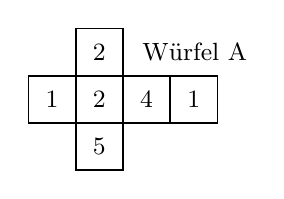
\begin{tikzpicture}[x=0.6cm,y=0.6cm,line width=0.6pt,baseline=(current bounding box.north)]\draw (1,2) rectangle ++(1,1); \node[font=\small] at (1.5,2.5) {2};\draw (0,1) rectangle ++(1,1); \node[font=\small] at (0.5,1.5) {1};\draw (1,1) rectangle ++(1,1); \node[font=\small] at (1.5,1.5) {2};\draw (2,1) rectangle ++(1,1); \node[font=\small] at (2.5,1.5) {4};\draw (3,1) rectangle ++(1,1); \node[font=\small] at (3.5,1.5) {1};\draw (1,0) rectangle ++(1,1); \node[font=\small] at (1.5,0.5) {5};\node[font=\small,anchor=south west] at (2.2,2.1) {Würfel A};\end{tikzpicture}\hspace{1cm}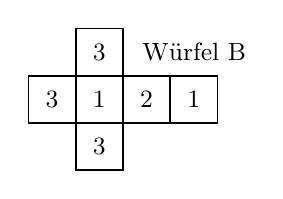
\begin{tikzpicture}[x=0.6cm,y=0.6cm,line width=0.6pt,baseline=(current bounding box.north)]\draw (1,2) rectangle ++(1,1); \node[font=\small] at (1.5,2.5) {3};\draw (0,1) rectangle ++(1,1); \node[font=\small] at (0.5,1.5) {3};\draw (1,1) rectangle ++(1,1); \node[font=\small] at (1.5,1.5) {1};\draw (2,1) rectangle ++(1,1); \node[font=\small] at (2.5,1.5) {2};\draw (3,1) rectangle ++(1,1); \node[font=\small] at (3.5,1.5) {1};\draw (1,0) rectangle ++(1,1); \node[font=\small] at (1.5,0.5) {3};\node[font=\small,anchor=south west] at (2.2,2.1) {Würfel B};\end{tikzpicture}\par
\end{pfaufg}
\begin{pfaufg}{}{a)}{1 BE}
Würfel A wird einmal geworfen. Gib die Wahrscheinlichkeit an, eine 2 zu würfeln.
\rechenplatz{3}
\fusshilfe{\mbox{Prüfstein a):~$\tfrac{2}{6}$ = $\tfrac{1}{3}$}}
\end{pfaufg}
\begin{pfaufg}{}{b)}{4 BE}
Erst wird Würfel A geworfen, dann Würfel B. Man achtet nur darauf, ob die Zahl gerade oder ungerade ist. Ergänze die Wahrscheinlichkeiten im Baumdiagramm. Ermittle die Wahrscheinlichkeit, dass beide Würfel eine ungerade Zahl zeigen.
\par\smallskip\noindent \begin{tikzpicture}[line width=0.5pt,baseline=(current bounding box.north)]\node[font=\scriptsize,mbgrau] at (2.04,0.70) {Würfel A};\node[font=\scriptsize,mbgrau] at (5.44,0.70) {Würfel B};\fill (0,-1.35) circle (1.3pt) coordinate (k0w);\node[font=\scriptsize,inner sep=2pt] (k1) at (3.40,-2.25) {ungerade};\node[font=\scriptsize,inner sep=2pt] (k0) at (3.40,-0.45) {gerade};\node[font=\scriptsize,inner sep=2pt] (k3) at (6.80,-0.90) {ungerade};\node[font=\scriptsize,inner sep=2pt] (k5) at (6.80,-2.70) {ungerade};\node[font=\scriptsize,inner sep=2pt] (k4) at (6.80,-1.80) {gerade};\node[font=\scriptsize,inner sep=2pt] (k2) at (6.80,0.00) {gerade};\draw[] (k0w) -- node[pos=0.55,anchor=north,draw,line width=0.3pt,fill=white,minimum width=0.7cm,minimum height=0.34cm,inner sep=0pt] {} (k1.west);\draw[] (k0w) -- node[pos=0.55,anchor=south,font=\scriptsize,fill=white,inner sep=1pt] {$\tfrac{3}{6}$} (k0.west);\draw[] (k0.east) -- node[pos=0.55,anchor=north,draw,line width=0.3pt,fill=white,minimum width=0.7cm,minimum height=0.34cm,inner sep=0pt] {} (k3.west);\draw[] (k1.east) -- node[pos=0.55,anchor=north,draw,line width=0.3pt,fill=white,minimum width=0.7cm,minimum height=0.34cm,inner sep=0pt] {} (k5.west);\draw[] (k1.east) -- node[pos=0.55,anchor=south,draw,line width=0.3pt,fill=white,minimum width=0.7cm,minimum height=0.34cm,inner sep=0pt] {} (k4.west);\draw[] (k0.east) -- node[pos=0.55,anchor=south,font=\scriptsize,fill=white,inner sep=1pt] {$\tfrac{1}{6}$} (k2.west);\end{tikzpicture}\par
\rechenplatz{3}
\fusshilfe{\mbox{Prüfstein b):~A ungerade $\tfrac{3}{6}$; B nach A gerade: ungerade $\tfrac{5}{6}$; $\tfrac{5}{12}$}}
\end{pfaufg}
\begin{pfaufg}{}{*c)}{2 BE}
Beide Würfel werden wie in b) geworfen. Bestimme die Wahrscheinlichkeit für das Ereignis E: „Nicht beide Würfel zeigen eine gerade Zahl.“
\rechenplatz{3}
\fusshilfe{\mbox{Prüfstein c):~$\tfrac{33}{36}$ = $\tfrac{11}{12}$}}
\end{pfaufg}
\begin{pfaufg}{}{*d)}{2 BE}
Auf Würfel B wird genau eine Zahl geändert. Dann werden beide Würfel nacheinander geworfen. Beschrifte das leere Netz von Würfel B (neu) so, dass die Summe 2 mit der Wahrscheinlichkeit $\tfrac{1}{6}$ fällt. Zeige mit einer Rechnung, dass deine Beschriftung passt.
\par\smallskip\noindent 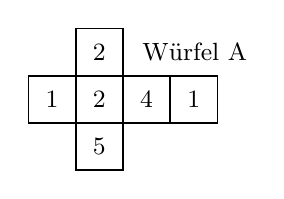
\begin{tikzpicture}[x=0.6cm,y=0.6cm,line width=0.6pt,baseline=(current bounding box.north)]\draw (1,2) rectangle ++(1,1); \node[font=\small] at (1.5,2.5) {2};\draw (0,1) rectangle ++(1,1); \node[font=\small] at (0.5,1.5) {1};\draw (1,1) rectangle ++(1,1); \node[font=\small] at (1.5,1.5) {2};\draw (2,1) rectangle ++(1,1); \node[font=\small] at (2.5,1.5) {4};\draw (3,1) rectangle ++(1,1); \node[font=\small] at (3.5,1.5) {1};\draw (1,0) rectangle ++(1,1); \node[font=\small] at (1.5,0.5) {5};\node[font=\small,anchor=south west] at (2.2,2.1) {Würfel A};\end{tikzpicture}\hspace{1cm}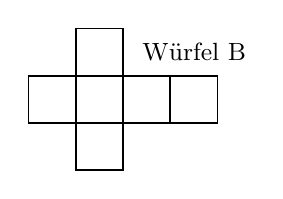
\begin{tikzpicture}[x=0.6cm,y=0.6cm,line width=0.6pt,baseline=(current bounding box.north)]\draw (1,2) rectangle ++(1,1); \node[font=\small] at (1.5,2.5) {};\draw (0,1) rectangle ++(1,1); \node[font=\small] at (0.5,1.5) {};\draw (1,1) rectangle ++(1,1); \node[font=\small] at (1.5,1.5) {};\draw (2,1) rectangle ++(1,1); \node[font=\small] at (2.5,1.5) {};\draw (3,1) rectangle ++(1,1); \node[font=\small] at (3.5,1.5) {};\draw (1,0) rectangle ++(1,1); \node[font=\small] at (1.5,0.5) {};\node[font=\small,anchor=south west] at (2.2,2.1) {Würfel B};\end{tikzpicture}\par
\rechenplatz{3}
\fusshilfe{\mbox{Prüfstein d):~$\tfrac{1}{6}$}}
\end{pfaufg}
\end{document}